%!TEX root = ../thesis.tex
%*******************************************************************************
%*********************************** First Chapter *****************************
%*******************************************************************************

\chapter{Introduction}  %Title of the First Chapter
\pagebreak
%s\doublespacing
\onehalfspacing

\section{Overview}

All organisms exist in a state of intense competition for resources. For many organisms, among the most dangerous competitors are parasites, which attempt to colonise the host's own body and co-opt its internal resources and systems to their own advantage. The evolutionary arms race between parasites and hosts is ancient, and has led to the development of a stunning variety of complex offensive and defensive adaptations on each side. % Mention faster evolution of parasites relative to hosts

Among the most complex and sophisticated systems developed as part of this ancient host/parasite conflict is the vertebrate adaptive immune system. By dynamically recombining their own DNA within specialised lymphocyte cells, jawed vertebrates are capable of producing an almost unlimited variety of different \textit{de novo} antigen-receptor proteins, and hence of responding effectively to entirely novel immune threats. In addition, by producing long-lived memory cells in response to antigenic stimulation, the adaptive immune system can retain the ability to respond to recurrent immune threats years or even decades after they were first encountered by an individual. This combination of dynamic adaptability to novel immune threats and persistent immune memory enables vertebrates to progressively improve their protection against predictable aspects of their immune environment, while also coping effectively with the rapid evolution which is one of the main advantages of bacterial and viral pathogens over their slower-evolving hosts.

Among the different branches of vertebrate adaptive immunity, the humoral immune system is unique in both the breadth of antigenic compounds it can respond to and its ability to produce secreted antigen-receptor proteins capable of acting independently of the cells that produced them. Whereas the T-lymphocytes of the cellular adaptive immune system can respond only to processed peptide antigens expressed on the surface of antigen-presenting cells, the antibodies produced by B-lymphocytes are capable of responding to almost any molecular structure on the surface of a cell or protein. Secreted antibodies in serum and mucosal secretions play a number of essential roles in vertebrate immunity, including opsonisation (recruitment of phagocytic cells), activation of complement, and inactivation and aggregation of antigens and pathogens, while membrane-bound antibodies (also known as B-cell receptors or BCRs) orchestrate B-cell development, and response to antigen exposure. An effective humoral immune system is essential to immune and organismal function in vertebrates, and mutations that disable humoral adaptive immunity in ...% species?
can lead to severe immunopathies and severely curtailed life expectancy. % TODO: Focus on importance here, move details to another section.

% TODO: Discuss antibodies specifically

Despite all its sophistication, however, the functionality of the vertebrate adaptive immune system declines dramatically with age, leaving older individuals increasingly vulnerable to infectious disease. In humans and other species, the decline in immune functionality with age manifests as a dramatic increase in deaths from infection in older people, as well as increasing levels of infection-associated morbidity and a decline in the effectiveness of pro-immune interventions such as vaccination. The molecular and physiological changes underlying this immunosenescent phenotype are wide-ranging, implicating many different parts of the immune system; however, a particularly important contributor is the systemic decline in the effectiveness of the adaptive immune system in % identifying and neutralising novel immune threats?
For the humoral adaptive immune system, established immunosenescent phenotypes include... % decline in naive B-cells, reduction of antibody avidity, increase in autoantibody production
% TODO: Recast in terms of humoral immunity *as part of* general immune phenotype

While fair amount is known about the cellular and physiological changes that take place in the humoral adaptive immune system with age in some species, much less is known about how these changes translate to alterations in the high-level diversity, clonal makeup, and other structural aspects of the overall antibody repertoire in older individuals. Such a high-level systemic approach to antibody diversity could potentially reveal a great deal about how ageing and other processes affect adaptive immune functionality in an organism. Specialised, high-throughput, quantitative approaches have been used to assess the structure, diversity and health of adaptive immune repertoires in various contexts, including development, disease, and ageing; in the latter case, this pre-existing work has revealed ... . However, much remains to be discovered about ... .

When it comes to investigating the ageing of vertebrate-specific adaptations like the adaptive immune system, research is made more difficult by a relative lack of well-suited model organisms. Most established short-lived model organisms used in ageing research (e.g. yeast, nematode worms, or fruit flies) are not vertebrates, while most established vertebrate models (e.g. zebrafish or \species{Xenopus}{laevis}) were selected for properties other than their lifespan (such as rapid development) and are too long-lived for use as ageing models in many contexts. Even mouse, the most widely-used vertebrate model organism for both ageing and other biomedical applications, has a median lifespan of several years in most commonly-used laboratory strains, making many ageing studies prohibitively expensive. 

In this context, the recent emergence of the turquoise killifish (\nfu), the shortest-lived vertebrate species currently bred in captivity, as a model organism for ageing research represents a highly promising development for the study of adaptive immunosenescence; ...

In this thesis, therefore, I establish the turquoise killifish as a model for the study of comparative immunology and humoral adaptive immunosenescence. 
, by characterising 

Using a combination of existing genomic assemblies and new sequence data, I assembled and characterised the immunoglobulin heavy chain (\igh{}) gene locus of the turquoise killifish and compared it to other newly-assembled loci from closely-related species, revealing a complex and rapidly-evolving ... with a number of surprisingly ideosyncratic features (\Cref{chap:locus}). Using the sequences from this newly-characterised locus, I established the first working immunoglobulin sequencing protocol in this species, which I used to investigate the diversity and complexity of heavy-chain immune repertoires in adult killifish and how this diversity changes with age in the whole body and the gut. The results of these investigations demonstrate that the turquoise killifish possesses a complex, diverse and individualised antibody repertoire, which undergoes a rapid decline in within-individual diversity and increase in between-individual variability with age. This phenomenon is particularly strong in the gut, with ..., and is likely to be an important contributor to the changes in gut microbiota structure and diversity observed in aged killifish. % TODO: Discuss lack of change from transfer?



\section{The vertebrate adaptive immune system} % Humoral? Teleost?

\subsection{Antibody structure and function}
\label{sec:intro_antibody_structure}

The lineage of lymphocytic white blood cells known as B-cells is ancient, with its origins predating any modern gnathostome (jawed-vertebrate) lineage and possibly the development of antibodies themselves \parencite{boehm2011design,kasahara2015vlr}. In modern jawed vertebrates, B-lymphocytes are responsible for the production, diversification and secretion of the antigen-receptor proteins known as antibodies \parencite{mix2006immunoglobulins,schroeder2010immunoglobulins}, as well as diverse other roles that vary between taxa \parencite{sunyer2013fishing}. In almost all species examined to date, antibodies share a common, and highly distinctive, tetrameric structure (\Cref{fig:intro-antibody-structure-schematic}), with two identical immunoglobulin heavy chains (IGH) and two light chains (IGL) linked by disulfide bonds into a roughly Y-shaped configuration \parencite{mix2006immunoglobulins,schroeder2010immunoglobulins}. The sequence and structure of these chains, and the corresponding regions of their underlying gene loci, is divided into an N-terminal (5') variable region and a C-terminal (3') constant region \parencite{mix2006immunoglobulins} (\Cref{fig:intro-antibody-structure-schematic}); together, the variable regions of each light/heavy-chain pair determines the antigen-binding specificity of the antibody, while the constant regions, particularly that of the heavy chain, determine its structure, functional properties, and interactions with the rest of the immune system \parencite{mix2006immunoglobulins,schroeder2010immunoglobulins}. Unsurprisingly, the sequence diversity of the constant region is far lower than that of the variable region, with most species expressing only a few distinct constant-region classes (or \textit{isotypes}) but an almost unlimited variety of variable region sequences (or \textit{ideotypes}).

As members of the immunoglobulin superfamily of proteins, the tertiary structure of antibody chains consists primarily of a species of immunoglobulin fold domains; most light chains consist of two such domains, while the number in heavy chains varies substantially with isotype \parencite{schroeder2010immunoglobulins}. In both heavy and light chains, the most N-terminal immunoglobulin fold comprises the variable region, while the rest make up the constant region (\Cref{fig:intro-antibody-structure-schematic}); in some taxa (but not in teleost fishes), one of the constant-region immunoglobulin folds is replaced with a flexible hinge domain in some isotypes to increase the flexibility of the heavy chain \parencite{schroeder2010immunoglobulins}. The three loops of the variable-region immunoglobulin fold facing the antigen-binding site are labelled H1, H2 and H3 in the heavy chain and L1, L2 and L3 in the light chain (\Cref{fig:intro-antibody-structure-loops}) and are principally responsible for determining the antigen-binding specificity of the antibody; their corresponding gene regions are known as complementarity-determining regions (CDRs) and are the main focus of sequence variability among ideotypes, while the other parts of the antibody sequence are known as framework regions (FRs or FWRs) and exhibit less variability \parencite{schroeder2010immunoglobulins}.

Most antibody isotypes can be expressed in secreted or membrane-bound form; in the latter case they are also known as B-cell receptors (BCRs) \parencite{bengten2015fishantibodies}. The choice between secreted and membrane-bound forms of an antibody is usually made through alternative splicing \parencite{bengten2015fishantibodies,mashoof2016immunoglobulins}; typically, the transmembrane domain and cytosolic tail of the BCR are expressed via two additional exons (TM1 and TM2). Other constant-region exons are referred to collectively as CH exons, and are numbered by their occurence in the protein chain from the variable region to the C-terminus. In secreted antibodies, the standard four-chain configuration described above is known as an antibody monomer \parencite{mix2006immunoglobulins}, while multiple four-chain antibodies bound together are referred to by the number of four-chain monomers they contain: dimers for two connected antibodies, tetramers for four, \etc \parencite{mix2006immunoglobulins,schroeder2010immunoglobulins} (\Cref{fig:intro-antibody-structure-multimers}). These multimeric antibody supercomplexes these complexes have increased overall avidity for antigen and so can respond more strongly to low levels of low-specificity antigen \parencite{mix2006immunoglobulins}; they can be bound together by covalent disulfide bonds between subunits \parencite{schroeder2010immunoglobulins} or, more rarely, by noncovalent intermolecular interactions \parencite{zhang2010igtgut}.

The number and variety of antibody heavy-chain classes available to B-cells in an organism, and the mechanism by which the isotype of an antibody is determined, vary substantially by species; in tetrapods, the isotype of the antibodies produced by a given B-cell can be modified by a specialised class-switch recombination (CSR) process which is absent in teleost fishes \parencite{senger2015switching}. Different isotypes vary in their length, flexibility, multimerisation behaviour (see below) and effector functions \parencite{schroeder2010immunoglobulins,senger2015switching}. In teleost fishes, three constant-region classes have been observed to date \parencite{bengten2015fishantibodies,mashoof2016immunoglobulins,fillatreau2013astonishing}:

\begin{itemize}
\item \textbf{Immunoglobulin M} (\igh{M}) was the first IgH isotype to be identified in teleosts \parencite{fillatreau2013astonishing}, and is homologous to the isotype of the same name found in mammals and other jawed vertebrates \parencite{mashoof2016immunoglobulins}. It is expressed in both secreted and transmembrane form \parencite{fillatreau2013astonishing}; in most teleosts, the transcript of the secreted form comprises four CH exons (\cm{1-4}), while the transmembrane form comprises three CH exons and two TM exons \parencite{bengten2015fishantibodies,fillatreau2013astonishing}. In contrast to mammals, in which secreted IGHM is primarily found as a pentamer, in teleosts it is typically found as a tetramer \parencite{fillatreau2013astonishing} connected by disulfide bonds between heavy chains \parencite{mashoof2016immunoglobulins}. In those fish species which have been tested, secreted IGHM is the main form of antibody found in serum \parencite{bengten2015fishantibodies,mashoof2016immunoglobulins,fillatreau2013astonishing}.
\item Like \igh{M}, \textbf{immunoglobulin D} (\igh{D}) is a primitive isoform present in most lineages of jawed vertebrates \parencite{mashoof2016immunoglobulins}, including teleost fishes. The size and structure of \igh{D} varies dramatically between teleost species, with the number of CH exons varying more than twofold, from roughly seven (\cd{1-7}) in some species to seventeen in zebrafish \parencite{mashoof2016immunoglobulins,fillatreau2013astonishing}. All teleost \igh{D} transcripts to date have possessed a chimeric \cm{1} exon from \igh{M}, a configuration almost unknown in mammals \parencite{mashoof2016immunoglobulins,fillatreau2013astonishing}; teleost \igh{D} also lacks the flexible hinge region present in mammalian \igh{D} \parencite{fillatreau2013astonishing}. A minority of teleost species have known secretory forms of \igh{D}, though the mechanism of producing them varies between species: in channel catfish, one dedicated sublocus has a dedicated IgD secretory exon in place of the transmembrane exons \parencite{bengten2006catfish}, while in rainbow trout (and possibly some other species like Atlantic salmon and cod) a run-on event at the end of \cd{7} results in the production of a secretory tail in a manner similar to secretory IgZ \parencite{ramirezgomez2012secretoryigd}. in other species, only transmembrane isoforms have been observed. In teleosts as in mammals, transmembrane \igh{D} is usually co-expressed with \igh{M}; however, its role in the adaptive immune system remains unclear \parencite{mashoof2016immunoglobulins}.
\item Unlike \igh{M} and \igh{D}, \textbf{immunoglobulin Z} (\igh{Z}, also known as \igh{T}, \igh{Z/T} and \igh{Z/T}) is unique to teleost fishes \parencite{fillatreau2013astonishing}. Also unlike \igh{M} and \igh{D}, \igh{Z} is not found universally among teleost loci -- of those IgH loci characterised to date, IgZ is missing in those of medaka and channel catfish \parencite{fillatreau2013astonishing,magadan2011medaka}, having apparently been lost independently in these species. In those species in which it is present, IgZ appears to act as a specialised mucosal antibody class, with elevated levels observed in mucosal secretions compared to the level in serum \parencite{zhang2010igtgut,fillatreau2013astonishing,xu2013igtskin}. Unlike teleost \igh{M}, secretory \igh{Z} in serum is predominantly monomeric, while in mucosal secretions it is found primarily as a tetramer bound together by noncovalent intermolecular bonds between heavy chains \parencite{zhang2010igtgut}. In most species, \igh{Z} comprises four CH exons (\cz{1-4}) and two TM exons \parencite{mashoof2016immunoglobulins}, though some species have fewer -- for example, stickleback \igh{Z} has only three CH exons \parencite{bao2010stickleback,gambondeza2011stickleback}, while fugu \igh{Z} has only two \parencite{fillatreau2013astonishing,savan2005fugu}.
\end{itemize}
% TODO: Figure links for this list?

\begin{figure}
\centering
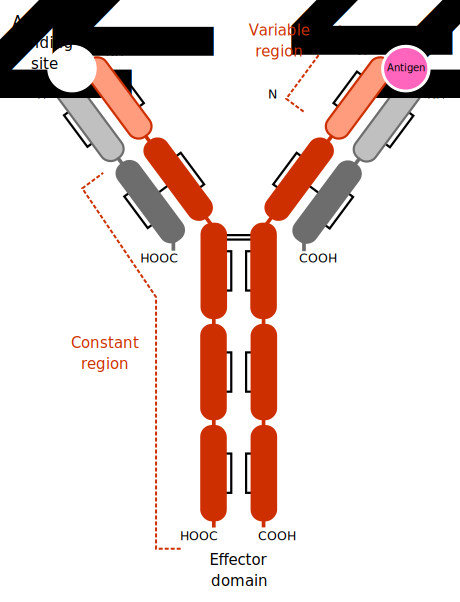
\includegraphics[width=0.9\textwidth]{_Figures/png_edited/antibody-structure}
\begin{subfigure}{0em}
\phantomsubcaption{}
\label{fig:intro-antibody-structure-schematic}
\end{subfigure}
\begin{subfigure}{0em}
\phantomsubcaption{}
\label{fig:intro-antibody-structure-loops}
\end{subfigure}
\begin{subfigure}{0em}
\phantomsubcaption{}
\label{fig:intro-antibody-structure-vdj}
\end{subfigure}
\begin{subfigure}{0em}
\phantomsubcaption{}
\label{fig:intro-antibody-structure-multimers}
\end{subfigure}
\caption[Antibody structure and function]{\textbf{Antibody structure and function:} (A) Schematic of a hingeless secreted antibody monomer, with heavy chains depicted in red, light chains in blue, and bound antigen in pink. Immunoglobulin fold domains are depicted as rounded rectangles, with variable-region domains shown with light shading and constant-region domains with dark. Black lines indicate disulfide bonds. (B) Schematic close-up of an immunoglobulin antigen-binding site, indicating the six loop regions (H1-3 and L1-3) making up the antigen-binding region. (C) Schematic close-up of the heavy-chain variable region, indicating the regions corresponding to the variable, diversity and joining gene segments from the unrecombined \igh{} locus. Note the chimeric nature of the third antigen-binding loop (H3, marked), which is formed by parts of all three gene segments. (D) In the context of antibodies, ``monomer'' refers to a single four-chain antibody protein, while ``dimer'', ``tetramer'' \etc refer to multiple antibodies linked together through covalent or noncovalent interactions.}
\label{fig:intro-antibody-structure}
\end{figure}
% TODO: Actual antibody crystal structure here?
% TODO: Discuss disulfide bonds in text
% TODO: Refer to VDJ schematic (1C) in next section

\subsection{Antibody sequence diversification and primary repertoire diversity}
\label{sec:intro_immunity_primary}

% TODO: Discuss allelic exclusion (Magadan)
% TODO: Discuss where primary and secondary diversification occur in fishes, and where B-cells reside (Mashoof)

The immune environment encountered by a vertebrate organism contains an enormous number of different potential pathogenic threats, each of which has its own antigenic signatures and many of which are capable of evolving much more rapidly than the vertebrate host. In order for the adaptive immune system to cope with this huge diversity of different threats, it must be able to produce antibodies with a correspondingly large diversity of different antigen specificities. The greater the potential diversity of antibody sequences available to the adaptive immune system, the greater its capacity to respond effectively to novel immune threats. In reality, the mechanisms employed by the vertebrate adaptive immune system to diversify its antigen receptors enable an almost unlimited diversity of potential antibody sequences, with a correspondingly vast array of potential antigen specificities.

The mechanisms by which the adaptive immune system produces this diversity are dramatic, and rely on a highly unusual underlying gene structure and a very high level of cellular wastage. In the humoral immune system, antibody diversification takes place during B-cell development in the primary lymphopoietic organs (bone marrow in mammals, anterior kidney in teleosts). Prior to this process, the native antibody loci in B-progenitor cells (and other cell types) is highly fragmented, with numerous fragmentary variable-region sequences present in series on the chromosome upstream of the constant-region exons. In the heavy chain locus, these variable-region gene segments can be divided into three categories:

\begin{itemize}
\item \textbf{Variable (\vh) segments} are the longest class of gene segment, at roughly \bp{300} in length. Each V-segment codes for the majority of the variable region of an antibody, including the entirety of the first three framework regions (FWR1-3) and the first two complementarity-determining regions (CDR1-2) as well as the 5' part of CDR3 \parencite{jung2006vdjr}. They are therefore highly structured, and include several highly-conserved positions present in virtually all functional V-segments in nearly all species, including two conserved cysteine residues (which code for an intra-domain disulfide bond) and a conserved tryptophan residue following CDR1. Each V-segment is also associated with its own promoter sequence and 5'-UTR, as well as a 5'/C-terminal leader peptide containing... % What does the leader do anyway? Trafficking signal?
\item \textbf{Diversity (\dh) segments} are the shortest class of segment, typically on the order of \bp{10}, and are the least structured. They form the middle part of CDR3.  % Like V-segments, D-segments are flanked by upstream promoter regions, which are involved in initiating the transcription required for DJ recombination. \parencite{jung2006vdjr}
\item \textbf{Joining (\jh) segments} are of intermediate length, typically 50-\bp{60}. They form the 3'/C-terminal part of heavy chain CDR3 and the 5'/N-terminal part of FR4. Each J-segment is succeeded on the chromosome by a splice donor site, which is used to join the variable region of the antibody sequence to the constant region via RNA splicing, following transcription of \igh{} mRNA. Like \vh segments, \jh segments can be identified from their conserved structure, particularly the conserved tryptophan residue marking the end of CDR3.
\end{itemize}

In the simplest translocon configuration of the \igh{} locus, blocks of repeated \vh, \dh and \jh segments are present in series on the chromosome in contiguous V-, D- and J-regions. During B-cell development, a single \vd, \dh and \jh segment are selected, and the intervening genomic regions are permanently excised from the genome to produce a single contiguous VDJ sequence coding for the complete variable region of an antibody. The mechanism by which this excision occurs is called VDJ recombination, and is fundamental to antibody sequence diversification. This process relies on recombination signal sequences (RSSs) flanking each variable gene segment in the unrecombined locus, which are recognised by a specialised recombinase complex formed by recombination-activating genes 1 and 2 (\gene{RAG1} and \gene{RAG2}). These RSSs possess a distinctive structure, with highly conserved heptamer and nonamer sequences separated by a spacer sequence of relatively unconserved sequence but conserved length (either 12 or \bp{23}, corresponding respectively to one or two turns of the DNA helix). Each functional \vh segment is succeeded by a \bp{23}-spacer RSS in 5'-3' orientation, while each \jh segment is preceded by a \bp{23}-spacer RSS in 3'-5' orientation; each \dh segment, meanwhile, is flanked by \bp{12}-spacer RSSs in 5'-3' and 3'-5' orientation, respectively. The recombinase complex binds pairs of RSSs with opposite orientation and dissimilar spacer lengths; as a result, D-J and V-D joins are permitted while V-J joins are prevented. % TODO: Add brief explanation of how join is made

% TODO: Order of recombinations: in mammals, in fish

VDJ recombination provides a basic combinatorial sequence diversity, with a number of possible sequences in the simplest case equal to the product of the numbers of \vh, \dh and \jh segments in the \igh{} gene locus. The number of potential \igh{} variable-region sequences in most species, however, is far higher than this, with an estimated ... possible sequences in humans and ... in mice. The difference arises as a consequence of the fact that the V/D and D/J joins produced by VDJ recombination are not exact, but instead involve a degree of terminal deletion and insertion of untemplated nucleotides at the segmental boundaries... % TODO: Explain insertions and deletions during VDJr

The insertions and deletions that occur at the V/D and D/J junctional boundaries during VDJ recombination vastly increase the potential sequence diversity of the heavy-chain CDR3 region, which as a consequence is by far the most important single region in determining antigen specificity. This junctional diversity, however, comes at a substantial cost. The indel mutations introduced by VDJ recombination are not constrained to occur in multiples of three or in the same number at each junction, resulting in a high rate of recombinations in which the \vh and \jh segments are out of frame with each other; still more loci are rendered nonfunctional through the introduction of \textit{de novo} STOP codons. As the sequence changes introduced by VDJ recombination are irreversible, many developing B-cells are left with permanently disrupted \igh{} loci on both chromosomes, and are left with no recourse but programmed cell death. In addition, the huge and untemplated sequence diversity introduced in this way means that some B-cells whose \igh{} loci do successfully undergo VDJ recombination are left with BCRs that either cannot effectively bind any antigen or strongly bind self-antigen, resulting in useless antibodies in the first case and a dangerous risk of autoimmunity in the second; these B-cells must be removed through a process of antigenic selection before \naive B-cells are permitted to exit the primary lymphopoietic organs, resulting in still more wastage as cells with nonfunctional or self-binding antigens undergo programmed cell death; if these selective processes are weakened by age or mutation, the rates of low-affinity or self-reactive antigens in the periphery will increase. % TODO: More detail on selection mechanisms
% TODO: Discuss primary B-cell selection to remove autoantibodies
% More details on primary selection in Kogut and its sources

The processes of VDJ recombination, junctional diversity and primary selection will produce a population of \naive B-cells with an extremely high diversity of heavy-chain ideotypes, with virtually every \naive B-cell expressing a unique variable-region sequence. Taken together, the resulting population of sequences represents the primary heavy-chain repertoire of the organism, and determines the range of different antigen sequences the humoral immune system of that organism can potentially respond to. The diversity of this primary repertoire depends on the native structure of the \igh{} locus in that species (which determines the number of segment choices available to the VDJ-recombination process), the distribution of possible numbers of insertions or deletions contributing to junctional diversity, and the stringency of the primary selection process.

%TODO: A similar, though less variable, process of sequence diversity occurs in the immunoglobulin light-chain loci of the developing B-cells, and the final pairing of heavy and light chains determines the ultimate functionality and specificity of the BCR in that lymphocyte.

\subsection{Affinity maturation and secondary repertoire diversity}

Following VDJ recombination and primary selection, developed \naive B-cells emerge from the primary lymphopoietic organs and circulate in the periphery. At some point, a subset of these \naive cells will make contact with their cognate antigen. If this contact occurs in the correct signalling context (in particular, in the presence of T-cell help), % TODO: Explain this better
the B-cell becomes activated and undergoes a clonal expansion process. During this proliferation, the B-cell's antibody genes undergo a very high rate of somatic mutation (known as somatic hypermutation or SHM), with mutations focused in the complementarity-determining regions coding for the antigen-binding loops of the variable region; in humans, ... % TODO: Rate of mutation
. This SHM process is orchestrated by the activation-induced cytidine deaminase enzyme (AID), which preferentially targets particular sequence motifs and deaminates cytidine residues to uracil. As a result, ... % TODO: Explain different mutations introduced by AID in SHM

The combination of clonal expansion and somatic hypermutation convert what was a single \naive B-cell into a \textit{clone} of related activated B-cells descended from a single \naive ancestor. These cells possess a range of similar but distinct heavy-chain sequences arising from SHM, which will vary in their affinity for the ancestral B-cell's cognate antigen. In order for clonal expansion and SHM to improve the adaptive immune system's ability to respond to that antigen, a selection process is needed to identify and advantage members of the clone with increased affinity for the antigen. This selection is effected through a competitive process in which clonally-expanded B-cells compete for an insufficient amount of cognate antigen on antigen-presenting cells (follicular dendritic cells in mammals, melanomacrophages in teleosts). Those cells which successfully bind antigen receive growth and differentiation signals, while those which do not undergo programmed cell death. As those cells with higher affinity for antigen are better able to outcompete other cells for antigen binding, this process increases the proportion of such cells in the clonal population, increasing its overall antigen affinity.

Clonal expansion, somatic hypermutation and clonal selection, collectively known as affinity maturation, result in both diversification and increased antigen affinity of antibodies following antigenic exposure. The processes making up affinity maturation are present in both mammals and teleost fishes; however, while teleost B-cells both undergo somatic hypermutation and exhibit increased antigenic affinity following initial exposure, this increase in affinity is typically far weaker (... % TODO: how much
) than that seen in mammals. The reasons for this difference are still not entirely clear, but appear to rest in a difference in the effectiveness of clonal selection between the two taxa... % TODO: Explain theory from AM paper
. As a result, while teleost B-cells proliferate and undergo clonal expansion in response to antigenic exposure, their ability to convert this into an increase in antigenic affinity is limited compared to mammals.

Following affinity maturation, activated B-cells undergo differentiation into memory cells (which persist in the bloodstream for long periods and provide secondary immune memory) and plasmablasts/plasma cells % TODO: What is the difference?
(which secrete large amounts of antigen to mount a powerful immune response). These derived cells can then undergo additional rounds of affinity maturation, resulting in even larger and more diverse clones and still higher levels of antigenic affinity. % TODO: Is this the right way round, or do additional rounds occur before differentiation?
In tetrapods, class switching between different constant-region isotypes also occurs as part of affinity maturation, and is also orchestrated by AID; however, this process is absent in teleosts.

The combination of the primary (\naive) repertoire described in \Cref{sec:intro_immunity_primary} with the clonal expansions and additional sequence diversity arising from affinity maturation constitutes the secondary heavy-chain repertoire of the organism. This is the repertoire actually encountered by incoming pathogens, and which we can sample directly through immune repertoire sequencing (...). % TODO: Reference here
In addition to the process underlying the diversity of the primary repertoire discussed in \Cref{sec:intro_immunity_primary}, the structure and diversity of the secondary repertoire depends on the degree of clonal expansion and hypermutation exhibited by B-cells in a given organism, the efficacy of clonal selection, and the relative abundance of different B-cell subtypes (which express different types and amounts of antibody) in the body at the time of the sample. Inferring the composition of the primary repertoire from that of the secondary is non-trivial, and requires an attempt to distinguish sequences arising from \naive versus activated B-cells or infer the former from the latter; once obtained, the \naive sequences can be used to infer the parameters of the generative process.

% TODO: Where do plasmablasts fit into this?

\subsection{\igh{} locus structure in teleost fishes}

In \Cref{sec:intro_immunity_primary} I described the process of \igh{} locus maturation in terms of an idealised translocon locus with a simple V-D-J--C region structure. In some species, including mice and humans, something close to this simplified structure actually obtains, albeit with greatly expanded V-regions. % TODO: Or "very large differences in the sizes of the different regions and the number of gene segments they contain"
In many species, however, this structure is a significant oversimplification of the actual layout of their \igh{} loci.

In teleost fishes, the simplest locus structures are exhibited by species such as zebrafish, ..., and fugu. In these species, the \igh{} locus adopts a V-D-J-\cz{}-D-J-\cm{}-\cd{} structure, with a single shared V-region followed by D- and J-regions specific to the \igh{Z} and \igh{M/D} constant regions, respectively. During VDJ recombination in these loci, the choice of D- and J-segments also determines the choice of constant region: if a pair of \dh and \jh segments upstream of the \igh{Z} constant region is selected, the cell will express \igh{Z}, while if the segments chosen are downstream of \igh{Z}, that constant region will be excised during VDJ recombination and \igh{M} and/or \igh{D} will be used instead. As a result, VDJ recombination in these species determines both the ideotype of a developing B-cell and its isotype.

While some teleost species, such as zebrafish, exhibit relatively simple \igh{} loci, many species exhibit much more complicated (and often much larger) locus structures. In many species, multiple distinct subloci (comprising V-, D- and J-regions and least one constant region) are present in tandem on the chromosome, often with distinct combinations of variable gene segments and constant regions... % Examples of very large or very complex (e.g. medaka or stickleback) constant regions
In some species, such as Atlantic salmon, whole-genome duplication has led to the existence of multiple distinct \igh{} loci on different chromosomes, each of which has its own complement of subloci, gene segments, and constant regions. In this mileau, pseudogenisation of gene segments or constant-region exons is common, resulting in some/many loci in which a minority of functional subloci are accompanied by a significant number of nonfunctional pseudogenes. % TODO: Is this exaggeration

...
% TODO: Discuss IGHZ-less species
% TODO: Discuss teleost IGH locus evolution
% TODO: Discuss difficulty of locus assembly

% TODO: Origins, methods and results of immune repertoire sequencing

% TODO: Adaptive immunosenescence in vertebrates and ageing of antibody repertoires

\section{Adaptive immunosenescence in mammals and teleosts} % TODO: Section or subsection? Do we actually know anything about teleosts here?

The immune system of aged vertebrates has long been known to undergo a severe and systemic decline with age \parencite{segre1977immunosenescence}. As a result of this decline, older individuals exhibit increased susceptibility to a wide range of bacterial, viral, and fungal infectious diseases, as well as higher rates of complications and mortality from those infections when they occur \parencite{sambhara2009vaccination}. In addition, the effectiveness of vaccination against these infections often declines dramatically in older individuals, with older individuals receiving half or less of the immune protection from vaccination exhibited by younger recipients \parencite{sambhara2009vaccination}. % TODO: More on general functional immunosenescence?

The increases in the incidence and severity of cancer and some autoimmune conditions observed in the elderly are also attributable to this generalised immunosenescent phenotype.


Taken together, these functional immunosenescent phenotype represent a major cause of morbidity and death in older individuals, in both humans and other vertebrate species.

Age-related changes in the humoral adaptive immune system are an essential contributor to the decline in immune functionality observed in older individuals. 

% Functional changes in B-cell immunity (seroprotection et cetera)

Diverse cellular and physiological changes have been reported that could underlie these functional changes in humoral immune function with age. 

In the bone marrow, aged mice exhibit significant declines in the number of B-cell progenitor and precursor cells, which also show decreases in proliferation capacity and an increase in rates of apoptosis \parencite{montecino2013immunosenescence,kogut2012bcells}. As a result, the rate of \naive B-cell output from the bone marrow is sharply reduced, falling as low as 10\% of its level in young mice \parencite{kogut2012bcells}. Combined with the longer lifespans of existing antigen-experienced cells in the periphery, ...

In both humans and mice, B-cells from older individuals exhibit impaired class-switch recombination capacity, possibly as a result of decreased AID expression \parencite{montecino2013immunosenescence,blomberg2013age}.

In humans, the absolute numbers of \naive and unswitched memory cells remain roughly constant in the periphery with age, while the number of class-switched memory cells declines \parencite{blomberg2013age}.

While memory-cell clones established early in life often persist into old age, \naive B-cells in aged humans demonstrate a severely reduced ability to give rise to new antigen-specific memory B-cells following antigenic stimulation, impairing the establishment of functional immune memory for novel threats \parencite{aberle2013mechanistic}.

In mice, the total number of B-cells in the periphery appears to be unchanged by ageing, while in human peripheral blood the number of B-cells declines with age \parencite{montecino2013immunosenescence,aberle2013mechanistic}. 

In mice, while the total number of B-cells does not appear to change with age \parencite{montecino2013immunosenescence}, the number of \naive B-cells resident in germinal centres declines, while the prevalence of antigen-experienced memory and plasma cells increases \parencite{mehr2011reversing,kogut2012bcells}. As these antigen-experienced B-cells have a longer lifespan than naive cells \parencite{kogut2012bcells}, they progressively dominate the B-cell repertoire of aged mice at the expense of \naive cells, while the pool of circulating immunoglobulins becomes progressively dominated by hypermutated antibodies specific to previously-encountered antigens \parencite{kogut2012bcells}. As these \naive cells are essential for responding to novel or mutated immune threats not previously encountered by the immune system, this change is thought to lead to a progressive reduction in the capacity of the humoral immune system to respond effectively to novel threats \parencite{kogut2012bcells}.



Older human individuals show a decrease in the number of plasmablasts developing as a result of vaccination \parencite{montecino2013immunosenescence}.

Older mice (?) also exhibit a reduced number and volume of germinal centres \parencite{mehr2011reversing}, a change which is ...

The antibodies themselves are also thought to decline in quality with age, with older individuals producing 

In humans, older individuals exhibit a substantially lower increase in antibody titre in response to vaccination \parencite{sasaki2011limited,aberle2013mechanistic}, a difference mainly arising from a decrease in the number of activated plasmablasts \parencite{sasaki2011limited,montecino2013immunosenescence}.

At least some of the declines in B-cell functionality with age are likely to be the result of age-related declines in the functionality of CD4\textsuperscript{+} T-cells, which are known to play a critical role in orchestrating the humoral immune response \parencite{montecino2013immunosenescence} and undergo severe age-related changes including reduced proliferation, dysregulated cytokine production and disrupted helper activity \parencite{aberle2013mechanistic}. The reduction in T-cell help in elderly individuals following vaccination 
has been implicated in the dramatic decline in the ability of these individuals to produce high titres of antigen-specific antibody in response to vaccination and other antigenic challenges \parencite{aberle2013mechanistic}.

In addition to changes in proliferation, differentiation and behaviour exhibited by aged B-cells, the quality of the antibodies they produce has also been reported to decline \parencite{montecino2013immunosenescence}. 

In mice, levels of somatic hypermutation appear to decline with age \parencite{henry2019influenza}, % More direct citation
while in humans... % More sources from Henry 2019
different sources have reported inconsistent trends \parencite{blomberg2013age}...

In humans, plasmablasts arising following influenza vaccination exhibit restricted somatic hypermutation, leading to impaired affinity maturation and reduced ability to adapt to changes in viral epitope structure \parencite{henry2019influenza}.

As a result, older humans are thought to exhibit a greater reliance on immune memory compared to the \naive repertoire, leading to impaired reperoire flexibility in response to novel or mutated antigens \parencite{henry2019influenza}.

At the level of the antibody repertoire, older individuals are believed to exhibit reduced diversity, with ...
Early techniques that investigated the repertoire by investigating the distribution of CDR3 lengths (CDR3 spetratyping) indicated that older humans frequently exhibit more distorted distributions dominated by CDR3 regions of a particular length, indicative of clonal expansion, and found that older individuals with more distorted spectratypes exhibited greater frailty and worse health and lifespan outcomes than those with more young-like spectratypes. % Cite Gibson here

In addition to being produced at lower titres in response to vaccination, anti-influenza antibodies produced by older human individuals demonstrate reduced ability to effectively neutralise viral haemagglutinin \parencite{sasaki2011limited,kogut2012bcells}, while antibodies produced by elderly subjects in response to pneumococcal polysaccharide vaccine demonstrate reduced opsonisation ability \parencite{kogut2012bcells}.

In primary responses to previously unseen yellow-fever vaccine, older individuals exhibit a significant delay in upregulation of antibody titres, and exhibit significantly higher levels of viral prevalence in the bloodstream during this delayed seroconversion period \parencite{kogut2012bcells}.

Aged humans exhibit progressive accumulation of increasing levels of self-reactive autoantibodies \parencite{kogut2012bcells}, possibly as a result of ...

% Discuss quality of bone marrow niche, reconstitution ability (Mehr), ability to transplant successfully (Kogut), etc?

% Role of HSC myeloid bias etc in reducing B-cell output (Kogut)


% Wang et al 2013
%Advanced age has been reported to lead to increased or de-
%creased B cell counts in the peripheral blood, increased, decreased
%or unchanged proportions of naive B cells, and increased CD5+
%B cell populations (3, 5, 9–13). Changes in serum Ab production,
%including decreases in vaccine-specific Abs, and decreased isotype
%switching associated with lower expression of activation-induced
%cytidine deaminase in B cells also have been described previously
%(8, 10, 14). Understanding the effects of aging on B cell function
%is further complicated by the common chronic viral infections
%seen at higher rates in the aging population, such as CMV and
%EBV. CMV infection is correlated with increased counts of LFA-
%1hiCD8+ memory T cells and reduced naive CD8+ T cells, whereas
%total B cell counts in the blood are reportedly increased in CMV-
%seropositive individuals (15–17).
%Following V(D)J rearrangement to generate functional Ig genes
%in B cells, the Ig repertoire during a human’s life span is further
%shaped by negative selection against self-Ags, clonal expansion of
%B cells stimulated by Ag, activation-induced mutation of Ig genes,
%and receptor editing, among other processes. Ineffective Ab re-
%sponses in the elderly have been attributed to decreased diversity
%of Ab repertoires with accumulation of memory B cells and de-
%crease of naive B cell populations (18). Influenza vaccination
%responses in the elderly are associated with decreased numbers of
%vaccine-stimulated B cells (8), and a recent study that included four
%elderly subjects show decreased diversity of influenza vaccine–
%stimulated B cells (19). However, there is also evidence of rela-
%tively preserved Ig repertoire diversity in tonsillar tissue of aged
%humans and increased proportions of naive B cells in some elderly
%individuals (20). Mutation of IGHV in B cell populations report-
%edly changes with aging, with one study reporting modestly in-
%creased mutation in IgG but not memory IgM B cell populations in
%the blood, whereas data from tonsillar B cells indicate increased
%mutation in memory IgM B cells but not other subsets (20, 21).
%Most prior studies of IGH gene rearrangements in young versus
%elderly subjects have been limited to examination of tens to hun-
%dreds of sequences, from small numbers of individuals, or have not
%assessed the potentially confounding effects of chronic herpesvirus
%infections (20–23). Seropositivity for CMV, in particular, increases
%with age in human populations and should be controlled for in
%studies of the effects of aging on the immune system (24).



% ... cellular/physiological changes

% Repertoire changes

% Limitation to a small number of species, small sample sizes, low spatial resolution, et cetera


%\section{Misc.}
%
%\subsection{Ageing of the antibody repertoire}
%
%% Notes from de Bourcey et al. (2017)
%.
%The vertebrate adaptive immune system has long been observed to undergo a severe decline with age in multiple species, with notable changes in humans including decreased lymphocyte proliferation \parencite{debourcy2017ageing} and defects in antibody production \parencite{debourcy2017ageing}. Changes in the human antibody repertoire observed with age include restricted
%
%In studies of peripheral blood repertoires taken before and after influenza vaccination, older individuals have been observed to show reduced within-individual and increased between-individual repertoire diversity \parencite{debourcy2017ageing}, suggesting that repertoires become increasingly (and divergently) specialised with age. Older repertoires also show less change in composition following vaccination, showing a reduced capacity to adapt to new information from the pathogenic environment \parencite{debourcy2017ageing}. An oligoclonal phenotype, in which one or a few memory B-cell lineages occupy a disproportionate share of repertoire diversity, has been reported in a subset of older individuals in multiple studies \parencite{debourcy2017ageing}; these expanded clones appear to be resistant to immunogenic interventions such as vaccination. 
%
%Within similarly-sized lineages, the repertoires of older individuals have been found to show reduced per-nucleotide sequence diversity, indicating an impairment in secondary diversification through somatic hypermutation; this effect is especially pronounced in larger clones \parencite{debourcy2017ageing}. % Fig 3D
%
%A subset of older repertoires also showed a greater prevalence of sequences bearing premature stop codons, indicating... % Also reduced "radical" mutations
%
%This loss in repertoire diversity with age is observed in both naive and antigen-experienced subsets of the repertoire \parencite{debourcy2017ageing}, but is strongest in the former, indicating an increase in the relative prevalence of the memory compartment within the repertoire. This is consistent with a model of the aged immune system as impaired by the accumulation of stubborn immune memory.
%
%An important feature of these studies is that CMV infection has been found to have an important influence of certain aspects of repertoire ageing, including...

%\section*{Summary} % Fits one one page if 1.5-spaced, but not at double spacing
%
%
%To understand and counter the complex changes that occur in the adaptive immune system with age, it is necessary to analyse the whole population of lymphocyte antigen-receptor sequences present in an individual. Such a top-down approach was impossible until relatively recently, when the advent of modern high-throughput sequencing technologies enabled the development of specialised protocols for immune-repertoire sequencing and analysis. Since then, the field of immune-repertoire studies has developed rapidly, providing a new and more powerful method for interrogating the changes ocurring in adaptive immune repertoires in a wide variety of contexts, including ageing. However, while initial human studies have indicated a decline in the diversity of these repertoires in older people, there remains a need for further research in this area. % This is weak, fill in once you've done your lit review.
%
%
%\pagebreak
%
%\section{The vertebrate adaptive immune system}
%
%
%
%\subsection{Mechanisms of heavy-chain diversification I: V(D)J recombination}
%
%
%% FIGURES AND TABLES:
%% - Schematic of native locus state -> VDJR -> recombined locus
%% - RAG structure and DNA Binding
%% - Schematic of RAG action and DNA excision
%% - Schematic of RSS structure
%% - Sequence logos of human/mouse/other RSSs
%% - Schematic of V/D/J coverage on protein chain
%% - Length distributions of human/mouse/other V/D/J segments
%
%The structure of the immunoglobulin heavy chain (\textit{IGH}) locus differs markedly between its native germline configuration and that adopted by a mature B-cell. In the native state, most \textit{IGH} loci comprise large numbers of isolated gene segments separated by non-coding DNA. These segments can be divided into three classes, variable (V), diversity (D) and joining (J), with distinct sequence properties and length distributions (see Box~\dots). % FIGURE: VDJ length distributions in humans etc; schematic of V/D/J positioning in peptide chain
%During B-cell development, site-specific recombination reactions result in the rearrangement of individual V, D and J segments into a continuous VDJ sequence, with the intervening genomic regions permanently excised and degraded. % Citation about what happens to excised sequences
%This irreversible genomic maturation process is known as V(D)J recombination.
%
%VDJ recombination is carried out by the RAG endonuclease complex, an enzyme formed by the association of \textbf{r}ecombination-\textbf{a}ctivating \textbf{g}enes 1 \& 2 \parencite{jung2006vdjr}. % more detailed citation, roles of RAG1 vs RAG2
%This complex, which is expressed specifically in developing lymphocytes, % citation needed
%introduces recognises specialised recombination sequences (RSSs) at the ends of IGH gene segments and introduces targeted double-strand breaks between two segments and their respective RSSs \parencite{jung2006vdjr}; these DSBs are then repaired by non-homologous end joining, resulting in a continuous coding sequence spanning both segments. The excised DNA ... % Citation for this
%
%VDJ recombination in the \textit{IGH} locus is highly structured, and occurs in a specific order. First, a D and a J segment are selected and recombined to produce a DJ sequence. Then, a V region is selected and recombined with the DJ to produce a continuous VDJ sequence constituting the variable region of the heavy chain. The complete protein sequence is produced during later transcriptional splicing, which joins this variable-region sequence to downstream constant-region exons to produce a mature \textit{IGH} mRNA. This strict ordering of V/D/J segments, which obtains in the vast majority of recombined sequences observed, is produced through the combination of a variety of regulatory mechanisms. The most basic of these is the structure of the RSSs, which comprise a conserved heptamer and nonamer sequence separated by a relatively unconserved spacer region of either 12 or 23bp \parencite{jung2006vdjr}, corresponding to either one or two turns of the DNA helix. V and J segments in the IGH locus are flanked by RSSs with 23bp spacer regions, while those flanking D-regions have 12bp spacers %citation needed
%As the RAG recombinase specifically recognises pairs of RSSs with dissimilar spacer lengths (a restriction known as the 12/23 or one-turn/two-turn rule), direct V-to-J recombination events are excluded \parencite{jung2006vdjr}. % Better citation if possible.
%
%In addition to the restrictions imposed by the 12/23 rule, additional limitations on VDJ recombination are imposed by the requirement that RAG binding be preceded by transcription from the to-be-recombined segments, apparently in order to open the chromatin structure in that region \parencite{jung2006vdjr}. Both V and D segments, but not J segments, are preceded by upstream promoter regions, which are involved in transcriptional initiation during specific stages of B-cell development...
%
%Complete VDJ recombination places the V-region promoter in close proximity to a highly-conserved enhancer element (known as iE$\mu$) lying between the last J segment and the first constant-region exon \parencite{jung2006vdjr}; this enhancer is important for strong expression of the mature IGH mRNA from the pre-B-cell stage onwards. 
%
%


%The mouse \textit{IGH} locus also adopts a translocon structure, in this case with an enormous V-region, comprising 150 or more V-segments (depending on the strain) spanning 2.7Mb \parencite{jung2006vdjr}. The 12-13 murine D segments occupy a region of approximately 50kb, while the four J segments cover about 2kb. This is followed by 200kb of constant region exons. 
%
%% Mouse locus (depending on strain): 150+ V, 12-13 D, 4 J. (\parencite{jung2006vdjr})
%% Total length of murine locus: ~3Mb near telomeric end of chr12
%
%\subsection{Antibody effector function and isotype diversity}
%
%
%
%\newpage
\section{The African turquoise killifish as a model for vertebrate ageing}
%
%% POSSIBLE FIGURES:
%% - Nothobranchius genus range, photos of different notho males
%% * Photo of male and female GRZ TK
%% * Lifespan curves of male and female GRZ-AD
%% - Diapause schematic
%% - Photograph of ephemeral pools in Zimbabwe
%% - Something showing correlation between aridity and lifespan in nothos
%% - Schematic comparing GRZ lifespan to other common ageing models, along with important present/absent human-like systems
%% - Phylogeny of TK within teleosts, with divergence times and human outgroup
%
%% POSSIBLE TABLES:
%% - List of notho species used in research with approx mean/max lifespans
%% - List of ageing phenotypes observed/not observed in GRZ / wild-derived strains
%% - Table of TK genome assemblies (JENA/STFD/CLGN) with metrics
%% - Comparison of genome metrics (size, repetitiveness, etc) between TK and other models
%% - Life history table for GRZ, MZM, other nothos, other fish models
%
The genus \textit{Nothobranchius} comprises a broad group of annual freshwater fishes distributed across equatorial and subequatorial Africa \parencite{valdesalici2003lifespan}, with species diversity concentrated in the south-east of the continent \parencite{genade2005annual}. Members of this genus share a suite of adaptations to life in ephemeral pools and rivers, most notably the production of desiccation-resistant embryos capable of surviving through the dry season in a diapause state \parencite{genade2005annual}. Fish from this genus have been known for several decades to  exhibit very rapid growth and short lifespans, consistent with their evolving under conditions of very high extrinsic mortality \parencite{valdesalici2003lifespan}, with many species exhibiting a median lifespan of less than one year. Nevertheless, there is wide variation within the genus in body size, growth rate and lifespan, with species from less arid regions tending to show slower growth and longer median lifespans \parencite{genade2005annual}.

Like other \textit{Nothobranchius} species, the turquoise killifish (\nfu) is a medium-sized annual fish first isolated from ephemeral freshwater pools -- in this case, from a relatively arid region of southeastern Zimbabwe \parencite{jubb1971new,genade2005annual}. Even by the standards of the \textit{Nothobranchius} genus, \Nfu exhibits extremely rapid growth, maturation, and ageing, with the most widely-used laboratory strain (GRZ) exhibiting a median lifespan of just 9-16 weeks \parencite{valdesalici2003lifespan,genade2005annual,terzibasi2008strains,kirschner2012map,valenzano2015genome,smith2017microbiota} -- the shortest lifespan of any captive-bred vertebrate, and a dramatic outlier on the distribution of vertebrate lifespans. % TODO: Adapt vertebrate lifespans figure from Smith 2017
Combined with their possession of several important vertebrate-specific adaptations -- including an adaptive immune system -- this extremely short lifespan makes the turquoise killifish a highly promising model organism for ageing research \parencite{harel2015crispr}.

Despite its very short lifespan, \textit{N. furzeri} has been found to show a wide range of senescent phenotypes in even the shortest-lived strains, including lipofuscin deposition \parencite{genade2005annual};  accumulation of senescence markers \parencite{genade2005annual};  increased neurodegenaration \parencite{valenzano2006resveratrol1,valenzano2006resveratrol2}; impaired learning and behavioural phenotypes  \parencite{genade2005annual,valenzano2006resveratrol1}; %loss of fecundity \parencite{api2018embryos,api2018fecundity}, %TODO: Published source for loss of fecundity in GRZ?
and a high incidence of degenerative and neoplastic lesions \parencite{dicicco2011histopathology}. These diverse phenotypes indicate that the short lifespan of the turquoise killifish is the result of an accelerated general ageing process, rather than the specific failure of a particular organ or system. Moreover, established anti-ageing interventions such as resveratrol treatment \parencite{valenzano2006resveratrol1}, reduction in ambient temperature \parencite{valenzano2006temperature} and dietary restriction \parencite{terzibasi2009dr} also extend lifespan in the turquoise killifish, indicating a strong analogy with the ageing phenotypes observed in canonical model systems.

Due primarily to its potential as a model organism for ageing research, the turquoise killifish has also seen rapid development as a genetic model. The short-lived GRZ strain has been bred in captivity for fifty years and at least a hundred generations \parencite{terzibasi2007review} and exibits a very high degree of homozygosity \parencite{reichwald2009genome,valenzano2009map,kirschner2012map}, providing a uniform genetic background for experimental interventions. A number of important genetic resources are now available, including several assemblies of the nuclear genome \parencite{reichwald2015genome,valenzano2015genome}, the most recent of which (in preparation) is of very high quality. These assemblies have revealed an unusually large genome for a teleost fish, with an estimated size of ... gigabases; % TODO: Cite new genome
This large size is primarily accounted for by the exceptionally high repeat content of the killifish genome, with at least ... percent of the genome composed of repetitive elements. % TODO: And again.
Karyotyping \parencite{reichwald2009genome} and sequencing analysis \parencite{reichwald2015genome} both indicate a chromosome number of $2n = 38$, corresponding to 19 distinct linkage groups in the haploid genome.

%Turquoise killifish are strongly sexually dimorphic, with an XY sex-determination system \parencite{reichwald2015genome,valenzano2009map} and large, colourful males. Most killifish studies to date have been performed using fish of only one sex, typically males; this thesis is no exception. TODO: Discuss dimorphism, sexual differences? (Maybe in discussion)

% TODO: Photo for thesis
%
%Phylogenetically, the genus \textit{Nothobranchius} falls within the Cyprinodontiformes, and the turquoise killifish is therefore closely related to a number of fish species that have been the subject of extensive research, including guppies, platyfish, medaka, sticklebacks, and pufferfish  \parencite{terzibasi2007review,hughes2018teleostphylo}. Conversely, the most well-developed teleost model organism, the zebrafish, is relatively distantly-related, with an estimated divergence time of over 200 Mya \parencite{hughes2018teleostphylo}, making the use in a killifish context of the many genetic and experimental resources developed for the zebrafish more challenging. As a result, techniques such as cell-type-specific cell sorting that depend on cell-surface markers or specific antibodies are often still unavailable for killifish studies, though many are under active development in one or more killifish laboratories.

% TODO: Round this off somehow